% Options for packages loaded elsewhere
\PassOptionsToPackage{unicode}{hyperref}
\PassOptionsToPackage{hyphens}{url}
%
\documentclass[
  12pt,
]{article}
\usepackage{amsmath,amssymb}
\usepackage{iftex}
\ifPDFTeX
  \usepackage[T1]{fontenc}
  \usepackage[utf8]{inputenc}
  \usepackage{textcomp} % provide euro and other symbols
\else % if luatex or xetex
  \usepackage{unicode-math} % this also loads fontspec
  \defaultfontfeatures{Scale=MatchLowercase}
  \defaultfontfeatures[\rmfamily]{Ligatures=TeX,Scale=1}
\fi
\usepackage{lmodern}
\ifPDFTeX\else
  % xetex/luatex font selection
    \setmainfont[]{Times New Roman}
\fi
% Use upquote if available, for straight quotes in verbatim environments
\IfFileExists{upquote.sty}{\usepackage{upquote}}{}
\IfFileExists{microtype.sty}{% use microtype if available
  \usepackage[]{microtype}
  \UseMicrotypeSet[protrusion]{basicmath} % disable protrusion for tt fonts
}{}
\makeatletter
\@ifundefined{KOMAClassName}{% if non-KOMA class
  \IfFileExists{parskip.sty}{%
    \usepackage{parskip}
  }{% else
    \setlength{\parindent}{0pt}
    \setlength{\parskip}{6pt plus 2pt minus 1pt}}
}{% if KOMA class
  \KOMAoptions{parskip=half}}
\makeatother
\usepackage{xcolor}
\usepackage[margin=1in]{geometry}
\usepackage{color}
\usepackage{fancyvrb}
\newcommand{\VerbBar}{|}
\newcommand{\VERB}{\Verb[commandchars=\\\{\}]}
\DefineVerbatimEnvironment{Highlighting}{Verbatim}{commandchars=\\\{\}}
% Add ',fontsize=\small' for more characters per line
\usepackage{framed}
\definecolor{shadecolor}{RGB}{248,248,248}
\newenvironment{Shaded}{\begin{snugshade}}{\end{snugshade}}
\newcommand{\AlertTok}[1]{\textcolor[rgb]{0.94,0.16,0.16}{#1}}
\newcommand{\AnnotationTok}[1]{\textcolor[rgb]{0.56,0.35,0.01}{\textbf{\textit{#1}}}}
\newcommand{\AttributeTok}[1]{\textcolor[rgb]{0.13,0.29,0.53}{#1}}
\newcommand{\BaseNTok}[1]{\textcolor[rgb]{0.00,0.00,0.81}{#1}}
\newcommand{\BuiltInTok}[1]{#1}
\newcommand{\CharTok}[1]{\textcolor[rgb]{0.31,0.60,0.02}{#1}}
\newcommand{\CommentTok}[1]{\textcolor[rgb]{0.56,0.35,0.01}{\textit{#1}}}
\newcommand{\CommentVarTok}[1]{\textcolor[rgb]{0.56,0.35,0.01}{\textbf{\textit{#1}}}}
\newcommand{\ConstantTok}[1]{\textcolor[rgb]{0.56,0.35,0.01}{#1}}
\newcommand{\ControlFlowTok}[1]{\textcolor[rgb]{0.13,0.29,0.53}{\textbf{#1}}}
\newcommand{\DataTypeTok}[1]{\textcolor[rgb]{0.13,0.29,0.53}{#1}}
\newcommand{\DecValTok}[1]{\textcolor[rgb]{0.00,0.00,0.81}{#1}}
\newcommand{\DocumentationTok}[1]{\textcolor[rgb]{0.56,0.35,0.01}{\textbf{\textit{#1}}}}
\newcommand{\ErrorTok}[1]{\textcolor[rgb]{0.64,0.00,0.00}{\textbf{#1}}}
\newcommand{\ExtensionTok}[1]{#1}
\newcommand{\FloatTok}[1]{\textcolor[rgb]{0.00,0.00,0.81}{#1}}
\newcommand{\FunctionTok}[1]{\textcolor[rgb]{0.13,0.29,0.53}{\textbf{#1}}}
\newcommand{\ImportTok}[1]{#1}
\newcommand{\InformationTok}[1]{\textcolor[rgb]{0.56,0.35,0.01}{\textbf{\textit{#1}}}}
\newcommand{\KeywordTok}[1]{\textcolor[rgb]{0.13,0.29,0.53}{\textbf{#1}}}
\newcommand{\NormalTok}[1]{#1}
\newcommand{\OperatorTok}[1]{\textcolor[rgb]{0.81,0.36,0.00}{\textbf{#1}}}
\newcommand{\OtherTok}[1]{\textcolor[rgb]{0.56,0.35,0.01}{#1}}
\newcommand{\PreprocessorTok}[1]{\textcolor[rgb]{0.56,0.35,0.01}{\textit{#1}}}
\newcommand{\RegionMarkerTok}[1]{#1}
\newcommand{\SpecialCharTok}[1]{\textcolor[rgb]{0.81,0.36,0.00}{\textbf{#1}}}
\newcommand{\SpecialStringTok}[1]{\textcolor[rgb]{0.31,0.60,0.02}{#1}}
\newcommand{\StringTok}[1]{\textcolor[rgb]{0.31,0.60,0.02}{#1}}
\newcommand{\VariableTok}[1]{\textcolor[rgb]{0.00,0.00,0.00}{#1}}
\newcommand{\VerbatimStringTok}[1]{\textcolor[rgb]{0.31,0.60,0.02}{#1}}
\newcommand{\WarningTok}[1]{\textcolor[rgb]{0.56,0.35,0.01}{\textbf{\textit{#1}}}}
\usepackage{longtable,booktabs,array}
\usepackage{calc} % for calculating minipage widths
% Correct order of tables after \paragraph or \subparagraph
\usepackage{etoolbox}
\makeatletter
\patchcmd\longtable{\par}{\if@noskipsec\mbox{}\fi\par}{}{}
\makeatother
% Allow footnotes in longtable head/foot
\IfFileExists{footnotehyper.sty}{\usepackage{footnotehyper}}{\usepackage{footnote}}
\makesavenoteenv{longtable}
\usepackage{graphicx}
\makeatletter
\newsavebox\pandoc@box
\newcommand*\pandocbounded[1]{% scales image to fit in text height/width
  \sbox\pandoc@box{#1}%
  \Gscale@div\@tempa{\textheight}{\dimexpr\ht\pandoc@box+\dp\pandoc@box\relax}%
  \Gscale@div\@tempb{\linewidth}{\wd\pandoc@box}%
  \ifdim\@tempb\p@<\@tempa\p@\let\@tempa\@tempb\fi% select the smaller of both
  \ifdim\@tempa\p@<\p@\scalebox{\@tempa}{\usebox\pandoc@box}%
  \else\usebox{\pandoc@box}%
  \fi%
}
% Set default figure placement to htbp
\def\fps@figure{htbp}
\makeatother
\setlength{\emergencystretch}{3em} % prevent overfull lines
\providecommand{\tightlist}{%
  \setlength{\itemsep}{0pt}\setlength{\parskip}{0pt}}
\setcounter{secnumdepth}{5}
% definitions for citeproc citations
\NewDocumentCommand\citeproctext{}{}
\NewDocumentCommand\citeproc{mm}{%
  \begingroup\def\citeproctext{#2}\cite{#1}\endgroup}
\makeatletter
 % allow citations to break across lines
 \let\@cite@ofmt\@firstofone
 % avoid brackets around text for \cite:
 \def\@biblabel#1{}
 \def\@cite#1#2{{#1\if@tempswa , #2\fi}}
\makeatother
\newlength{\cslhangindent}
\setlength{\cslhangindent}{1.5em}
\newlength{\csllabelwidth}
\setlength{\csllabelwidth}{3em}
\newenvironment{CSLReferences}[2] % #1 hanging-indent, #2 entry-spacing
 {\begin{list}{}{%
  \setlength{\itemindent}{0pt}
  \setlength{\leftmargin}{0pt}
  \setlength{\parsep}{0pt}
  % turn on hanging indent if param 1 is 1
  \ifodd #1
   \setlength{\leftmargin}{\cslhangindent}
   \setlength{\itemindent}{-1\cslhangindent}
  \fi
  % set entry spacing
  \setlength{\itemsep}{#2\baselineskip}}}
 {\end{list}}
\usepackage{calc}
\newcommand{\CSLBlock}[1]{\hfill\break\parbox[t]{\linewidth}{\strut\ignorespaces#1\strut}}
\newcommand{\CSLLeftMargin}[1]{\parbox[t]{\csllabelwidth}{\strut#1\strut}}
\newcommand{\CSLRightInline}[1]{\parbox[t]{\linewidth - \csllabelwidth}{\strut#1\strut}}
\newcommand{\CSLIndent}[1]{\hspace{\cslhangindent}#1}
\usepackage{tcolorbox}
\usepackage{amssymb}
\usepackage{yfonts}
\usepackage{bm}
\usepackage{titlesec}
\usepackage{kbordermatrix}


\newtcolorbox{greybox}{
  colback=white,
  colframe=blue,
  coltext=black,
  boxsep=5pt,
  arc=4pt}
  
\newcommand{\sectionbreak}{\clearpage}

 
\newcommand{\ds}[4]{\sum_{{#1}=1}^{#3}\sum_{{#2}=1}^{#4}}
\newcommand{\us}[3]{\mathop{\sum\sum}_{1\leq{#2}<{#1}\leq{#3}}}

\newcommand{\ol}[1]{\overline{#1}}
\newcommand{\ul}[1]{\underline{#1}}

\newcommand{\amin}[1]{\mathop{\text{argmin}}_{#1}}
\newcommand{\amax}[1]{\mathop{\text{argmax}}_{#1}}

\newcommand{\ci}{\perp\!\!\!\perp}

\newcommand{\mc}[1]{\mathcal{#1}}
\newcommand{\mb}[1]{\mathbb{#1}}
\newcommand{\mf}[1]{\mathfrak{#1}}

\newcommand{\eps}{\epsilon}
\newcommand{\lbd}{\lambda}
\newcommand{\alp}{\alpha}
\newcommand{\df}{=:}
\newcommand{\am}[1]{\mathop{\text{argmin}}_{#1}}
\newcommand{\ls}[2]{\mathop{\sum\sum}_{#1}^{#2}}
\newcommand{\ijs}{\mathop{\sum\sum}_{1\leq i<j\leq n}}
\newcommand{\jis}{\mathop{\sum\sum}_{1\leq j<i\leq n}}
\newcommand{\sij}{\sum_{i=1}^n\sum_{j=1}^n}
	
\usepackage{bookmark}
\IfFileExists{xurl.sty}{\usepackage{xurl}}{} % add URL line breaks if available
\urlstyle{same}
\hypersetup{
  pdfauthor={Jan de Leeuw - University of California Los Angeles},
  hidelinks,
  pdfcreator={LaTeX via pandoc}}

\title{Smacof at 50: A Manual\\
Part 8: Homogeneity Analysis}
\author{Jan de Leeuw - University of California Los Angeles}
\date{Started April 13 2024, Version of July 05, 2024}

\begin{document}
\maketitle
\begin{abstract}
smacofHO
\end{abstract}

{
\setcounter{tocdepth}{3}
\tableofcontents
}
\textbf{Note:} This is a working manuscript which will be expanded/updated
frequently. All suggestions for improvement are welcome. All Rmd, tex,
html, pdf, R, and C files are in the public domain. Attribution will be
appreciated, but is not required. The files can be found at
\url{https://github.com/deleeuw} in the repositories smacofCode, smacofManual,
and smacofExamples.

\section{Introduction: Categorical Data}\label{introduction-categorical-data}

In this chapter we shall analyze categorical data structures, with the following components.

\begin{itemize}
\tightlist
\item
  There are \(m\) \emph{variables}.
\item
  Variable \(j\) has \(k_j>1\) \emph{categories}.
\item
  There are \(n\) \emph{objects}.
\item
  Each object defines a \emph{partial order} over the categories of each variable. Make this the simple tree.
\end{itemize}

Introduce indicators

Discuss: separation and compactness. Start with MSA and De Leeuw (1969),
De Leeuw (2004), De Leeuw (2003)

Thus the actual data we collect are the \(n\times m\) partial orders \(\lesssim_{ij}\).

We study minimization of the stress \emph{loss function}
\begin{equation}
\sigma(X,Y_1,\cdots,Y_m):=\sum_{j=1}^m\sum_{i=1}^n\min_{\hat d_i^j\in\Delta_i^j}\sum_{l=1}^{k_j}w_{il}^j(\hat d_{il}^j-d_{il}(X,Y_j))^2
\label{eq:snmu}
\end{equation}
over the \(n\times p\) matrix of \emph{object scores} \(X\), the \(k_j\times p\)
matrices of \emph{category scores} \(Y_j\), and the \(n\times k_j\) \emph{transformations} (or \emph{optimal scalings}) \(\Delta_j\). We write
\(d_{il}(X,Y_j)\) for the distance between object \(i\) and category
\(l\) of variable \(j\). Note that for each variable \(j\) there are different matrices of category scores \(Y_j\), but there is only a single matrix of object scores \(X\).

The \(w_{il}^j\) in definition \eqref{eq:snmu}
are non-negative \emph{weights}. Formulas and derivations simplify if the data are \emph{row-weighted}, by which we mean that \(w_{il}^j=w_i^j\). They simplify
even more if weights are \emph{constant}, i.e.~if all non-zero weights
are equal to one.

The transformations in \eqref{eq:snmu}
are \emph{row-conditional}, in the sense that for each \(i\) a vector
\(\hat d_i^j\) of length \(k_j\) is selected by the technique
from a cone of admissible transformations \(\Delta_i^j\). Each row has its own cone.

We need a few words to discuss the meaning of the word ``model'' in this
context, since it is used frequently in data analysis. The
model corresponding with a loss function \(\sigma\) is the set of parameter
values for which \(\sigma\) attains its global minimum (usually zero).
Thus a model is a system of equations and/or inequalities.
In the case of loss function \eqref{eq:snmu} the model is
that the \(d_{il}(X,Y_j)\) with \(w_{il}^j>0\) satisfy the partial order \(\lesssim_{ij}\). Define
\begin{equation}
\epsilon^j_{il\nu}:=
\begin{cases}
1&\text{ if we require }\hat d^j_{il}\lesssim\hat d^j_{i\nu},\\
0&\text{ otherwise}
\end{cases}
\end{equation}
Then the model is the system of inequalities
\begin{equation}
w_{il}^jw_{i\nu}^j\epsilon^j_{il\nu}(d_{il}(X,Y_j)-d_{i\nu}(X,Y_j))\geq 0
\label{eq:model}
\end{equation}

If the cones \(\Delta_i^j\) contain the zero vector, then the global minimum of loss function \eqref{eq:snmu} is clearly equal to zero. Collapsing all \(x_i\) and all \(y_l^j\) into a single point makes all distances zero, and thus makes stress zero. There is also zero stress if we collapse all \(x_i\) into one point and all \(y_l^j\) into another point. These solutions are \emph{trivial} in the sense that, although they satisfy the model, they are
independent of the data and consequently not informative. There are also more subtle
trivial solutions.
Suppose the cones \(\Delta_i^j\) contain the set of all non-negative constant vectors. Collapse all \(x_i\) into a single point, and place all \(y_l^j\) for variable \(j\) on a sphere around the point \(x_i\). There can be different radii for different variables. This makes all \(d(x_i,y_l^j)\) equal to the radius of the sphere and thus makes stress zero.

In the context of non-metric unfolding there has been much work
on avoiding trivial and degenerate solutions. This started as soon as
Kruskal-Guttman-type iterative MDS techniques using data transformation became available. Early contributions were Roskam (1968) and Kruskal and Carroll (1969). For valuable summaries of more recent work, mostly by Willem Heiser and his students, we refer to the dissertations of Van Deun (2005) and Busing (2010).

It follows from the existence of these trivial solutions that we cannot define the purpose of our algorithms as finding the minimum of \eqref{eq:snmu} over all \(\hat D_j\), \(X\) and \(Y_j\). Some constraints on the optimization problems are needed to prevent these trivial or degenerate solutions.

\section{Homogeneity Analysis}\label{hom}

The \emph{Gifi System} (Gifi (1990), Michailidis and De Leeuw (1998), De Leeuw and Mair (2009)) implements non-linear or non-metric versions of the classical linear multivariate analysis techniques (regression, analysis of variance, canonical analysis, discriminant analysis, principal component analysis). The non-linear versions are introduced as special cases of \emph{Homogeneity Analysis}, which is better known as \emph{Multiple Correspondence Analysis}.

In this section we present homogeneity analysis as a technique for
minimizing the loss function \eqref{eq:snmu} when the data are \(n\times k_j\) \emph{indicator matrices} \(G_j\), with \(j=1,\cdots,m\). This is a non-standard presentation, because usually homogeneity analysis is related to principal component analysis, and not to multidimensional scaling
(see, for example, De Leeuw (2014) or De Leeuw (1923)). Hoffman and De Leeuw (1992)

In homogeneity analysis the data are (or are coded as) \(m\) \emph{indicator matrices} \(G_j\), where \(G_j\) is \(n\times k_j\).
Indicator matrices are binary matrices, with rows that add up to one or to zero.
Thus each row has either a single element equal to one and the rest zeroes, or it has all elements equal to zero. Indicator matrices are
used to code our categorical variables. Rows corresponds with objects
(or individuals), columns with the categories (or levels) of a variable.
Element \(g_{il}^j\) is one if object \(i\) is in category \(l\) of variable \(j\), and all other elements in row \(i\) are zero. If an object is \emph{missing} on variable \(j\) then the whole row is zero.

Homogeneity analysis makes joint maps in \(p\) dimensions of objects
and categories, both represented as points. A joint map for variable \(j\)
has \(n\) object points \(x_i\) and \(k_j\) category points \(y^j_{il}\).
In a homogeneous solution the object points are close to the points of the categories that the objects score in, i.e, to those \(y^j_{il}\) for which \(g^j_{il}=1\). If there is only one variable then it is trivial to make a perfectly homogeneous map. We just make sure the object points coincide with their category points. But there are \(j>1\) indicator matrices, corresponding with \(m\) categorical variables, and there is only a single set of object scores. The solution is a compromise trying to achieve as much homogeneity as possible for all variables simultaneously.

In loss function \eqref{eq:snmu} applied to homogeneity analysis
the sets \(\Delta_i^j\) are defined in such a way that \(\hat d_{il}^j\) is zero if \(i\) is in category \(l\) of
variable \(j\). There are no constraints on the other \(\hat d\)'s in row \(i\)
of variable \(j\). Thus for zero loss we want an object to coincide with all \(m\) categories it is in. With this definition of the \(\Delta_i^j\) we have
\begin{equation}
\min_{\hat d_i^j\in\Delta_i^j}\sum_{l=1}^{k_j}w_{il}^j(\hat d_{il}^j-d(x_i,y_l^j))^2=f_{ij}d_{ij}^2(X,Y),
\label{eq:homsnmu}
\end{equation}
where
\begin{subequations}
\begin{align}
d_{ij}(X,Y)&:=\sum_{l=1}^{k_j}g_{il}^jd(x_i,y^j_l),\label{eq:dred}\\
f_{ij}&:=\sum_{l=1}^{k_j}w^j_{il}w^j_{il}.\label{eq:wred}
\end{align}
\end{subequations}
Note that the \(w^j_{il}\) for which \(g^j_{il}=0\) play no role in
homogeneity analysis. In the usual implementations of homogeneity
analysis and multiple correspondence analysis
\(f_{ij}\) is either zero or one, depending on whether observation
\(i\) on variable \(j\) is missing or non-missing.

Using indicator matrices we can write loss function \eqref{eq:homsnmu} as
\begin{equation}
\sigma(X,Y_1,\cdots,Y_m)=
\sum_{j=1}^m\text{tr}\ (X-G_jY_j)'F_j(X-G_jY_j),
\label{eq:matsnmu}
\end{equation}
The \(F_j\) are diagonal matrices with the \(f_{ij}\) from \eqref{eq:wred}
on the diagonal.

In homogeneity analysis we minimize \eqref{eq:matsnmu} using the
explicit normalization \(X'F_\star X=I\), where \(F_\star\) is the
sum of the \(F_j\). The solution is given by the singular value
equations
\begin{subequations}
\begin{align}
X\Lambda&=F_\star^{-1}\sum_{j=1}^m F_jG_jY_j,\label{eq:homsvd1}\\
Y_j&=(G_j'F_jG_j)^{-1}G_j'F_jX,\label{eq:homsvd2}
\end{align}
\end{subequations}
where \(\Lambda\) is a symmetric matrix of Lagrange multipliers.

In homals (Gifi (1980), De Leeuw and Mair (2009)) alternating least squares is used
to solve the equations \eqref{eq:homsvd1} and \eqref{eq:homsvd2}. We start with
some initial \(X\), then compute the corresponding \(Y_j\) using \eqref{eq:homsvd2},
then for these new \(Y_j\) we compute a new corresponding \(X\) from \eqref{eq:homsvd1},
and so on. Computations are efficient, because only diagonal matrices need to
be inverted and matrix multiplication with an indicator matrix is not really multiplication but simply selection of a particular row or column. Alternating least squares thus becomes \emph{reciprocal averaging}. Equation \eqref{eq:homsvd2} says that the optimal category
point is the weighted averages of the objects points in the category, and \eqref{eq:homsvd1}
says that, except for rescaling with the Lagrange multipliers, the optimal object
point is the weighted average of the category points that the object scores in.

Alternative methods of computation (and interpretation) are possible if we
substitute \eqref{eq:homsvd2} in \eqref{eq:homsvd1} to eliminate the \(Y_j\)
and obtain an equation in \(X\) only. This gives
\begin{equation}
F_\star X\Lambda=\sum_{j=1}^m F_jG_j(G_j'F_jG_j)^{-1}G_j'F_jX,
\label{eq:geneigx}
\end{equation}
which is a generalized eigenvalue equation for \(X\). If we substitute \eqref{eq:homsvd1}
in \eqref{eq:homsvd2} we obtain generalized eigenvalue equations for \(Y\).
\begin{equation}
(G_j'F_jG_j)Y_j\Lambda=\sum_{h=1}^m G_j'F_jW_\star^{-1}F_hG_hY_h.
\label{eq:geneigy}
\end{equation}
If \(k_\star\), the sum of the \(k_j\), is not too large then finding the \(p\) largest non-trivial eigenvalues with corresponding eigenvectors from \eqref{eq:geneigy} may be computationally efficient. The largest ``trivial'' eigenvalue is always equal to one, no matter what the \(G_j\) and \(W_j\) are, and we can safely ignore it. The trivial solution with all distances equal to zero mentioned in section \ref{snmu} corresponds with this largest eigenvalue.

Homogeneity analysis can be most convincingly introduced using the concept of a \emph{star plot}. For variable \(j\) we plot \(k_j\) category points and \(n\) object
points in a single joint plot. We then draw a line from each category point to the points of the objects in that category. This creates \(k_j\) groups of
lines and points in \(\mathbb{R}^p\), and each of these groups is called a \emph{star}.
The sum of squares of the line lengths of a star is the loss of homogeneity for category \(l\) of variable \(j\), and the total sum of squares of all line lengths in the \(k_j\) stars is the loss \eqref{eq:matsnmu} for variable \(j\). Homogeneity analysis chooses \(X\) and the \(Y_j\) such that \(X\) is normalized by \(X'F_\star X=I\) and the stars are as small or as compact as possible, measured by the squared line lengths. For given \(X\) the stars are as small as possible by choosing the category points \(Y_j\) as the centroids of the object points in the category, as in equation
\eqref{eq:homsvd2}. That explains the use of the word ``star'', because now the stars really look like stars. In graph theory a star is a tree with one internal node (the category point) and \(k\) leaves (the object points). Thus, given the optimum choice of the \(Y_j\) as centroids, we can also say that homogeneity analysis quantifies the \(n\) objects in such a way that the resulting stars are as small as possible.

\section{Multidimensional Structuple Analysis MSA}\label{multidimensional-structuple-analysis-msa}

The Guttman-Lingoes series of programs (Lingoes (1973))
discusses, among many others, several techniques for analyzing
a number of indicator matrices. They have the acronyms
MSA-I, MSA-II, MSA-III, and MSA-IV, where MSA is short for
either Multidimensional Scalogram Analysis or Multidimensional
Structuple Analysis. Unfortunately the techniques are rather
poorly documented in the mainstream literature. I rely on Lingoes (1968b),
Lingoes (1968a), Lingoes (1972), Lingoes (1979), and the various
short program descriptions Lingoes published in Behavioural Science.
Unfortunately I currently have no access to Lingoes (1973).

All MSA programs start their iterations with MAC-II. MAC stands for
Multivariate Analysis of Contingencies, and the technique implements
the equations from Guttman (1941). In other words, MAC is homogeneity
analysis or multiple correspondence analysis. Thus the MSA
programs have the same starting configuration as our smacof
programs for categorical data.

The publications on MSA do not pay much attention to the existence
of trivial solutions and to the speed of convergence of the
iterations.

\subsection{MSA-I}\label{msa-i}

The most interesting member of the MSA sequence is MSA-I.

\begin{quote}
The logic of MSA-I was worked out by Guttman as a creative reaction to a number of objections to other proposed solutions for multidimensional scalogram analysis raised by members of his course on multidimensional analysis during his visit to The University of Michigan (1964-1965).
Some of the computational details and the programming of the technique were done by the author. (Lingoes (1968a), p.~76)
\end{quote}

The most complete description of MSA-I is probably Zvulun (1978). There
are also some computational details in Lingoes (1968a). So what is this
MSA-I model ?

Partition the object points corresponding to any category A into inner and outer points. Take any point not in A and find the closest point in A to that point. Such a closest point is called an \emph{outer point} of category A. Go through all points not in A to find all outer points of A. The points of A that are not outer points of A are \emph{inner points} of A.
Category A is \emph{contiguous} if each inner point of A is closer to an outer point of A than to any other outer point. Since the closest point in B to an inner point of A is by definition an outer point of B we have also contiguity if and only if each inner point of A is closer to some outer point of A than to any point outside A.

In MSA-I there are no category points, only object points. This makes
comparison with the partitioning by Voronoi regions complicated. In
the same way there is no obvious connection with the convex hulls of
the object points in a category. Separations and partitions can be quite
irregular and in the various small examples I have seen are mostly
done after the fact by hand.

The algorithm to optimize contiguity is described in (\textbf{lingoes\_68?}). I will
try to reconstruct it.

\subsection{MSA-II}\label{msa-ii}

Unlike MSA-I, MSA-II, which seems to be mostly due to Lingoes, is
pretty straightforward. The model, as taken from Lingoes (1968a), is that
there is a \(\rho>0\) such that \(g_{il}^j=1\) implies \(d(x_i,y_l^j)\leq\rho\)
and \(g_{il}^j=1\) implies \(d(x_i,y_l^j)\geq\rho\). Geometrically:

\begin{itemize}
\tightlist
\item
  circles with center \(x_i\) and radius \(\rho\) contain all categories
  object \(i\) scores in, all other category points are outside the circle
\item
  circles with center \(y_l^j\) and radius \(\rho\) contain all objects that score in category \(l\) of variable \(j\), all other object points are
  outside the circle.
\end{itemize}

Computionally we interpret the \(n\times k_\star\) binary supermatrix
\((G_1\mid\cdots\mid G_m)\) as a matrix of similarities and apply
a non-metric MDS technique. The data consist of two tie-blocks,
the ones and the zeroes, and we use the primary approach to ties.
Observe there is no row-conditionality here and there is only a single
radius \(\rho\).

The loss function for MSA-II is simply Kruskal's stress formula one,
implicitely normalized by the sum of all \(n\times k_\star\)
distances, with monotone regression replaced by rank images.

This use of rank images, by the way, is somewhat problematic.
There are \(nm\) smallest distances, corresponding with the
elements of \(G\) equal to one, and \(n(k_\star-m)\) largest distances.
But how do we define the rank images within the two tie blocks ?
Lingoes ranks the distances within the tie blocks from small to large, which seems rather arbitrary.

\subsection{MSA-III}\label{msa-iii}

MSA-III is closer to our smacofHO method.

\section{The smacofHO Loss Function}\label{the-smacofho-loss-function}

The smacofHO technique solves the closely related problem in which we do not require, as in homogeneity analysis, that
\begin{subequations}
\begin{equation}
\sum_{l=1}^{k_j}g^j_{il}\hat d^j_{il}=0
\label{eq:homcons}
\end{equation}
for all $i$ and $j$, but we impose the weaker condition that for all $i$ and $j$
\begin{equation}
\sum_{l=1}^{k_j}g^j_{il}\hat d^j_{il}\leq\hat d^j_{i\nu}
\label{eq:hocons}
\end{equation}
\end{subequations}
for all \(\nu=1,\cdots,k_j\).
In homogeneity analysis the geometric interpretation of loss is that we
want objects to coincide with all categories they score in. The geometric interpretation of loss function \eqref{eq:snmu} is that we want
objects to be closer to the categories they score in than to the categories
they do not score in.

This can be formalized using the notion of \emph{Voronoi regions}. The Voronoi region of
category \(l\) of variable \(j\) is the polyhedral convex set of all points of \(\mathbb{R}^p\) closer to category \(l\) than to any other category of variable \(j\). The plot of the the \(k_j\) categories of variable \(j\) defines \(k_j\) Voronoi regions that
partition \(\mathbb{R}^p\). For a wealth of information about Voronoi regions we refer to

Loss function \eqref{eq:snmu} with \(\Delta\) defined by constraint\eqref{eq:hocons} vanishes if for each variable all \(x_i\) are in the Voronoi regions of the categories they score in. This condition implies, by the way, that the interiors of the \(k_j\) convex hulls of the \(x_i\) in a given category are disjoint, and the point clouds can consequently be weakly separated by hyperplanes. Since the category points themselves are in their own Voronoi region the convex hulls of the stars are also disjoint.

The initial configuration for the iterations is computed using homogeneity analysis. In each iteration configuration updates are alternated with updates of the \(\hat D_j\).
The general majorization theory for MDS with restrictions (De Leeuw and Heiser (1980)) calls for configuration updates
in two steps. In the first step we compute the Guttman transform of the current configuration, and in the second step we project the Guttman transform on the set of constrained configurations.

Minimizing loss \eqref{eq:snmu} over the \(\hat d_i^j\) is a monotone regression problem for a simple tree order. This is easily solved by using Kruskal's primary approach to ties (Kruskal (1964a), Kruskal (1964b), De Leeuw (1977)).

\subsection{The Guttman Transform}\label{the-guttman-transform}

The smacof iterations, or Guttman transforms, more or less ignore the fact that we are dealing with a rectangular matrix and use the weights to transform the problem into a symmetric one (as in Heiser and De Leeuw (1979)).

The loss function is
\begin{equation}
\sigma(Z_1,\cdots,Z_m)=\sum_{j=1}^m\sum_{i=1}^{n_j}\sum_{k=1}^{n_j}w_{ik}^j(\hat d_{ik}^j-d_{ik}(Z_j))^2,
\label{eq:fullloss}
\end{equation}
with \(n_j:=n+k_j\) and with \(Z_j\) the \(n_j\times p\) matrices that stack \(X\) on top of
\(Y_j\). The \(w_{ik}^j\) are zero for the diagonal \(n\times n\) and the diagonal
\(k_j\times k_j\) block.

To compute the Guttman transform of \(Z_j\) we have to solve
the partitioned system
\begin{equation}
\begin{bmatrix}
R_W&-W\\
-W'&C_W
\end{bmatrix}
\begin{bmatrix}\tilde X\\\tilde Y\end{bmatrix}=
\begin{bmatrix}
R_B&-B\\
-B'&C_B
\end{bmatrix}
\begin{bmatrix}X\\Y\end{bmatrix}
\label{eq:guttman}
\end{equation}
Since we have to solve this system for each variable separately we forget about the index \(j\) here. In
\eqref{eq:guttman} \(R_W\) and \(C_W\) are the diagonal matrices with row and column sums of \(-W\), while \(R_B\) and \(C_B\) are diagonal matrices with the row and columns sums of the \(n\times k_j\) matrix \(B\), which has elements
\begin{equation}
b_{il}=w_{il}\frac{\hat d_{il}}{d_{il}(X,Y_l)}.
\label{eq:bdef}
\end{equation}
Matrices \(X\) and \(Y\) are the two parts of the current \(Z\) that we are updating,
while we solve for \(\tilde X\) and \(\tilde Y\), the two parts of the Guttman
transform.

Define
\begin{equation}
\begin{bmatrix}
P\\Q
\end{bmatrix}:=
\begin{bmatrix}
R_B&-B\\
-B'&C_B
\end{bmatrix}
\begin{bmatrix}X\\Y\end{bmatrix}
\label{eq:gusolve}
\end{equation}
Now
\(R_W\tilde X-W\tilde Y=P\) or \(\tilde X=R_W^{-1}(P+W\tilde Y)\). Substitute this in \(C_W\tilde Y-W'\tilde X=Q\)
to get \(C_W\tilde Y-W'R_W^{-1}(P+W\tilde Y)=Q\) or
\begin{equation}
(C_W-W'R_W^{-1}W)\tilde Y=Q+W'R_W^{-1}P
\label{eq:solvefory}
\end{equation}
We solve equation \eqref{eq:solvefory} for \(\tilde Y\) and then use \(\tilde X=R_W^{-1}(P+W\tilde Y)\).
Note that \(C_W-W'R_W^{-1}W\) is doubly-centered.
As in homogeneity analysis we hope that \(k_\star\)
is not to big, and we avoid generalized inverses of very large and very
sparse matrices.

\subsection{The smacof Projection}\label{the-smacof-projection}

After computing the Guttman transforms \(\tilde X_j\) and \(\tilde Y_j\) we have to project them on the set of constrained configurations.

First suppose the only constraint is \(X_j=X\). We will discuss some additional (optional) constraints in a while. To project we must minimize
\begin{multline}
\sum_{j=1}^m\text{tr}\ (X-\tilde X_j)'R_j(X-\tilde X_j)-2\sum_{j=1}^m\text{tr}\ (X-\tilde X_j)'W_j(Y_j-\tilde Y_j)+\\
\sum_{j=1}^m\text{tr}\ (Y_j-\tilde Y_j)'C_j(Y_j-\tilde Y_j)
\end{multline}
where \(R_j\) and \(C_j\) are now the diagonal matrices of row and column sums of the \(W_j\).

The stationary equations are
\begin{align}
Y_j&=\tilde Y_j-C_j^{-1}W_j'(X-\tilde X_j),\label{eq:stateq1}\\
X&=\{R_\star\}^{-1}\sum_{j=1}^m\left\{R_j\tilde X_j-W_j(Y_j-\tilde Y_j)\right\}.\label{eq:stateq2}
\end{align}
We solve these equations iteratively using alternating least squares.
This means using \eqref{eq:stateq1} to compute a new \(Y\) for given \(X\) and \eqref{eq:stateq2} to compute a new \(X\) for given \(Y\). We alternate these two updates until convergence.

Thus we have an iterative ``inner'' ALS process within the iterative
``outer'' ALS process of alternating the Guttman transform/projection and the monotone regressions. More precisely the inner iterations are in the
projection phase of the Guttman update.

If there are further constraints on \(X\), besides \(X_j=X\), and if there
are constraints on \(Y_j\) the updates in the projection phase must
be modified.

\subsubsection{Rank Constraints for Y}\label{rank-constraints-for-y}

If ww choose to do we can require the \(Y_j\) to have rank \(r_j\leq\min(k_j,p)\), i.e.~\(Y_j=Q_jA_j'\)
with \(Q_j\) a \(k_j\times r_j\) matrix and \(A_j\) a \(p\times r_j\) matrix.
The rank-constraint on \(Y_j\) is taken from the Gifi system, where it serves to connect homogeneity analysis with forms of non-linear principal
component analysis.

If \(r=1\) then geometrically having all \(y_l^j\) on a line through the origin implies that all Voronoi boundaries are hyperplanes perpendicular to that line, and consequently all Voronoi regions are bounded by two parallel hyperplanes (parallel lines if \(p=2\)). All objects scores must orthogonally project on the line in the interval corresponding with the category theyscore in. Note that the intervals on the line are actually the one-dimensional Voronoi regions of the line with the category points.

If \(r=2\) and \(p=3\), another case that may be practically relevant, then category points are in a hyperplane through the origin. The Voronoi regions in three-dimensional space are bounded by lines perpendicular to that plane, intersecting the plane at the two-dimensional Voronoi points for that plane. The object points must be in the correct polyhedral cylinder.

For each of the \(m\) variables we can independently choose the ranks \(r_j\) of the \(Y_j\) and combine it with one of the three options for \(X\), creating a large number of different analyses (in a given dimensionality \(p\)).

If there are rank constraints on one of more of the \(Y_j\) then for those \(j\) we have to minimize
\[
2\text{tr}\ A_j'\{Y_j'C_j-(X-\tilde X_j)'W_j\}Q_j+
\text{tr}\ A_j'Q_j'C_jQ_jA_j
\]
The stationary equations are
\[
\{Y_j'C_j-(X-\tilde X_j)'W_j\}Q_j=Q_j'C_jQ_jA_j,
\]
and
\[
\{Y_j'C_j-(X-\tilde X_j)'W_j\}'A_j=C_jQ_jA_jA_j'
\]

\subsubsection{Centroid Constraints on Y}\label{centroid-constraints-on-y}

If we require that \(Y_j=(G_j'R_jG_j)^{-1}G_j'R_jX\) then this effectively eliminates the \(Y_j\) as variables from the optimization problem and we only have to optimize over \(X\). We must minimize
\begin{multline}
\sum_{j=1}^m\text{tr}\ (X-\tilde X_j)'R_j(X-\tilde X_j) -
\text{tr}\ (X-\tilde X_j)'W_j(H_jX-\tilde Y_j)+\\
\text{tr}\ (H_jX-\tilde Y_j)'C_j(H_jX-\tilde Y_j)
\end{multline}
Expanding
\begin{multline}
2\ X'R_\star X-2\ \text{tr}\ X'\sum_{j=1}^mR_j\tilde X_j-2\ \text{tr}\ X'\{\sum_{j=1}^mW_jH_j\}X + 2\text{tr}\ X'\sum_{j=1}^mW_j\tilde Y_j+\\
\text{tr}\ X'\{\sum_{j=1}^mH_j'C_jH_j\}X-2\text{tr}\ X'\{\sum_{j=1}^mH_j'C_j\tilde Y_j\}
\end{multline}

Substituting \(Y_j=H_jX\) with \(H_j:=(G_j'R_jG_j)^{-1}G_j'R_j\) in .. and simplifying gives
the stationary equations \(P_\star X= Q_\star\) with
\begin{subequations}
\begin{align}
P_\star&:=\sum_{j=1}^m\{R_j-H_j'W_j'-W_jH_j+H_j'C_jH_j\},\\
Q_\star&:=\sum_{j=1}^m\{(R_j-H_j'W_j')\tilde X_j-(W_j-H_j'C_j)\tilde Y_j\}.
\end{align}
\end{subequations}
Thus the unnormalized solution for the object scores is \(X=P^+_\star Q_\star\).

We want to avoid inversion of the matrix \(P_\star\), which has order \(n\). In fact we do not want to compute and store \(P_\star\) at all. huppel

We avoid the inversion by using majorization. Suppose \(\mu\) is such that \(P_\star\lesssim\mu R_\star\) in the Loewner sense. We would typically take \(\mu\) as the largest eigenvalue of \(R_\star^{-1}P_\star\).

Define
\[
\omega(X):=\text{tr}\ X'P_\star X-2\ \text{tr}\ X'Q_\star
\]
Then, reculer pour mieux sauter, writing \(\overline{X}\) for the current best
\(X\),
\[
\omega(X)=\text{tr}\ (\overline X+(X-\overline X))'P_\star(\overline X+(X-\overline X))-2\ \text{tr}\ (\overline X+(X-\overline X))'Q_\star
\]
Now
\begin{multline}
\omega(X)\leq\omega(\overline X)+
\mu\text{tr}\ (X-\overline X)'R_\star(X-\overline X)-2\ \text{tr}\ (X-\overline X)'(Q_\star-P_\star\overline X)
\end{multline}
The stationary equations in the unnormalized case have solution
\[
X=\overline X+\mu^{-1}R_\star^{-1}(Q_\star-P_\star\overline X)
\]
If we require the normalization \(X'R_\star X=I\) then we must solve the Procrustus problem
\[
(\mu R_\star-P_\star)\overline X - Q_\star=R_\star X\Lambda
\]
with \(\Lambda\) a symmetric matrix of Lagrange multipliers.

\subsubsection{Normalization of X}\label{normalization-of-x}

Besides \(X_j=X\) we can also optionally require the normalization constraint \(X'R_\star X=I\). In both cases the stationary equation \eqref{eq:stateq1} remains the same, while \eqref{eq:stateq1} becomes
\[
R_\star X\Lambda=P_\star,
\]
with
\[
P_\star:=\sum_{j=1}^m\left\{R_j\tilde X_j-W_j(Y_j-\tilde Y_j)\right\}
\]
and with \(\Lambda\) a symmetric matrix of Lagrange multipliers.
Using the symmetric square root, \(\Lambda=(P'R_\star^{-1}P)^\frac12\) and thus
\[
X=R_\star^{-1}P(P'R_\star^{-1}P)^{-\frac12}.
\]
Thus requiring normalized object scores only needs small modifications in the \(X\) update step of the unnormalized update \(R_\star^{-1}P\).

\section{Convergence and Degeneracy}\label{convergence-and-degeneracy}

\section{Utilities}\label{utilities}

\subsection{Object Plot Function}\label{object-plot-function}

\subsection{Category Plots Function}\label{category-plots-function}

\subsection{Joint Plot Function}\label{joint-plot-function}

\subsection{Prediction Table}\label{prediction-table}

In the solution \((X,Y)\) we say that pair \((i,j)\) is a \emph{hit} if
\[
d_{il}^j(X,Y)=\min_{\nu=1}^{k_j}d_{i\nu}^j(X,Y)
\]
or, in words, if object point \(x_i\) is in the Voronoi region of the category point
corresponding to the category the object scores in.

\section{Examples}\label{examples}

Since there are so many different analyses that can be done (choosing
the rank and normalization constraints), and since each analysis leads
to a large number of plots, presentation of results is a problem. We encourage readers to repeat the analyses we present and study the output
in more detail.

\subsection{Small}\label{small}

We start we a small artificial example, earlier used for illustrative purposes in Gifi (1990), chapter 2. The data have \(n=10\) objects and
\(m=3\) variables with 3, 3, 2 categories.

\begin{verbatim}
##    first second third
## 01     a      p     u
## 02     b      q     v
## 03     a      r     v
## 04     a      p     u
## 05     b      p     v
## 06     c      p     v
## 07     a      p     u
## 08     a      p     v
## 09     c      p     v
## 10     a      p     v
\end{verbatim}

We first give the Voronoi + star joint plots for a homogeneity
analysis of the data, using the function \texttt{smacofHomogeneityHO()}.

\begin{figure}

{\centering 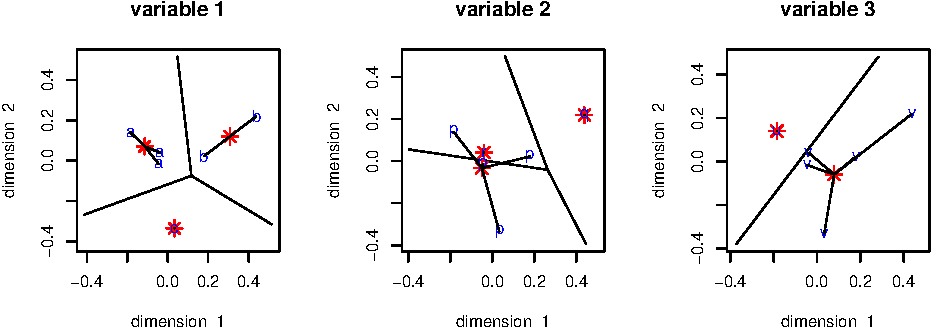
\includegraphics{smacofHO_files/figure-latex/smallhomals-1} 

}

\caption{Small example, Homogeneity Analysis}\label{fig:smallhomals}
\end{figure}

The solution is Voronoi homogeneous for variables one and three. For
variable two the star for category \(p\) has objects in the Voronoi
region of category \(r\), and is consequently not perfectly homogeneous.
This also shows in the prediction table from this analysis.

\begin{verbatim}
##       [,1] [,2] [,3]
##  [1,]    1    0    1
##  [2,]    1    1    1
##  [3,]    1    1    1
##  [4,]    1    0    1
##  [5,]    1    0    1
##  [6,]    1    1    1
##  [7,]    1    0    1
##  [8,]    1    1    1
##  [9,]    1    1    1
## [10,]    1    1    1
\end{verbatim}

Note that varable \(p\) is atypical, because eight of the ten objects
are in category \(p\), while \(q\) and \(r\) only have a single object
in them.

We next use the Homogeneity Analysis solution as intial estimate
for a smacof analysis without normalization or rank constraints.
Stress is \ensuremath{1.1313536\times 10^{-9}} after 169 iterations.

\begin{figure}

{\centering 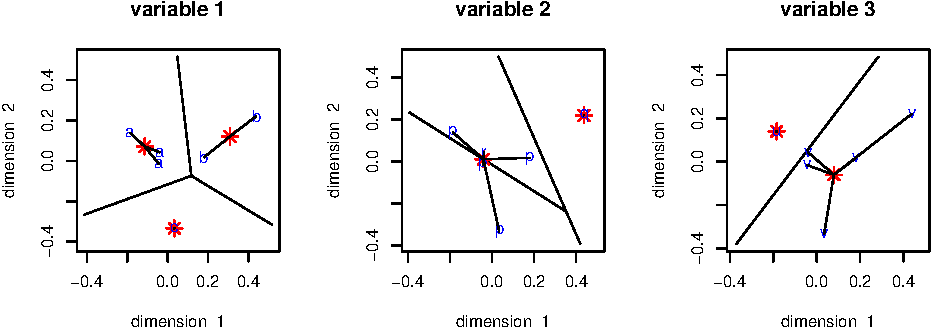
\includegraphics{smacofHO_files/figure-latex/smallplot00-1} 

}

\caption{Small example, smacofHO unrestricted}\label{fig:smallplot00}
\end{figure}

As expected, variables one and three, which already has perfect fit, do not change. There is some change in variable two, in the right
direction, but it is not enough to improve the number of correct
predictions.

\begin{verbatim}
##       [,1] [,2] [,3]
##  [1,]    1    0    1
##  [2,]    1    1    1
##  [3,]    1    1    1
##  [4,]    1    0    1
##  [5,]    1    0    1
##  [6,]    1    1    1
##  [7,]    1    0    1
##  [8,]    1    1    1
##  [9,]    1    1    1
## [10,]    1    1    1
\end{verbatim}

Finally, for this example, we constrain the \(Y_j\) to be of rank one
and leave \(X\) unnormalized. Stress is \ensuremath{4.3071361\times 10^{-10}} after 73 iterations.

\begin{figure}

{\centering 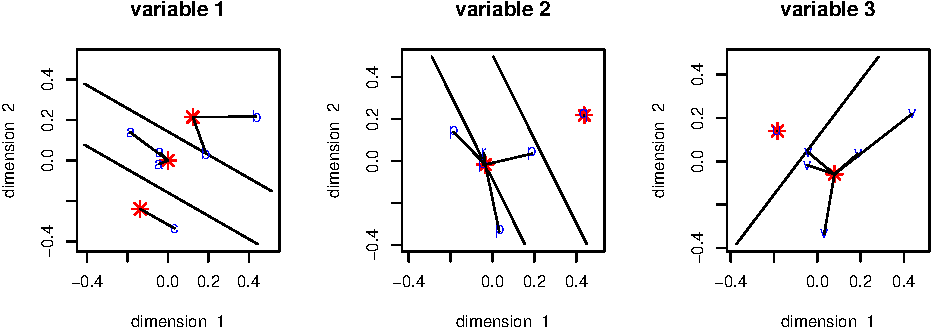
\includegraphics{smacofHO_files/figure-latex/smallplot10-1} 

}

\caption{Small example, smacofHO rank one}\label{fig:smallplot10}
\end{figure}

Variable three, which is binary, does not change. The plot for variable two changes for the better. To improve the fit the algorithm moves the
category points for categories \(p\) and \(r\) very close together. There is
still one prediction violation in variable two, but
if the category points of \(p\) and \(r\) coincide they have the same Voronoi
region and the prediction violation disappears. This may happen if we
continue iterating. The same is true for the prediction violation in
variable one, where object five in category \(b\) is very close to the
boundary between \(a\) and \(b\).

\begin{verbatim}
##       [,1] [,2] [,3]
##  [1,]    1    1    1
##  [2,]    1    1    1
##  [3,]    1    1    1
##  [4,]    1    1    1
##  [5,]    0    0    1
##  [6,]    1    1    1
##  [7,]    1    1    1
##  [8,]    1    1    1
##  [9,]    1    1    1
## [10,]    1    1    1
\end{verbatim}

We do note that the constrained version does better than the
unconstrained version. But this merely means that the constrained
version finds a better local minimum -- both analyses do not
find the global minimum, which we know is equal to zero.

\subsection{Cetacea}\label{cetacea}

Our first real example has \(m=15\) variables and \(n=37\) objects. The
objects are genera of whales, dolphins, and porpoises . The variables are morphological, osteological, and behavioral descriptors,
all categorical with a small number of categories. They are

\begin{verbatim}
##                                    [,1]
## NECK                                  2
## FORM OF THE HEAD                      6
## SIZE OF THE HEAD                      2
## BEAK                                  4
## DORSAL FIN                            4
## FLIPPERS                              4
## SET OF TEETH                          5
## FEEDING                               4
## BLOW HOLE                             4
## COLOR                                 5
## CERVICAL VERTEBRAE                    2
## LACRYMAL AND JUGAL BONES              3
## HABITAT                               5
## LONGITUDINAL FURROWS ON THE THROAT    3
## HEAD BONES                            5
\end{verbatim}

The data matrix has been constructed by Vescia (1985). Chapter 1 of the
book edited by Marcotorchino, Proth, and Janssen (1985) has the data, and a number of sub-chapters in which different data analysts
apply various techniques to these data and discuss the results. Among the contenders were Multidimensional Structuple Analysis (Guttman (1985))
and homals (Van der Burg (1985)).

\begin{Shaded}
\begin{Highlighting}[]
\NormalTok{hcethom }\OtherTok{\textless{}{-}} \FunctionTok{smacofHomogeneityHO}\NormalTok{(cetacea)}
\NormalTok{hcetho }\OtherTok{\textless{}{-}} \FunctionTok{smacofHO}\NormalTok{(cetacea, }\AttributeTok{verbose =} \ConstantTok{FALSE}\NormalTok{, }\AttributeTok{itmax =} \DecValTok{10000}\NormalTok{)}
\end{Highlighting}
\end{Shaded}

Stress is \ensuremath{5.9054624\times 10^{-8}} after 3417 iterations.

\begin{Shaded}
\begin{Highlighting}[]
\FunctionTok{smacofObjectsPlotHO}\NormalTok{(hcethom, }\AttributeTok{cex =}\NormalTok{ .}\DecValTok{5}\NormalTok{)}
\end{Highlighting}
\end{Shaded}

\pandocbounded{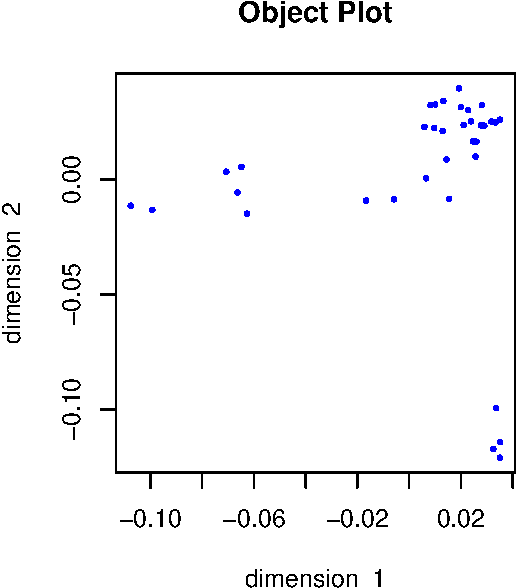
\includegraphics[keepaspectratio]{smacofHO_files/figure-latex/cetaplot-1.pdf}}

\begin{Shaded}
\begin{Highlighting}[]
\NormalTok{hcethompre }\OtherTok{\textless{}{-}} \FunctionTok{smacofPredictionTable}\NormalTok{(hcethom)}
\FunctionTok{print}\NormalTok{(}\FunctionTok{colSums}\NormalTok{(hcethompre, }\AttributeTok{na.rm =} \ConstantTok{TRUE}\NormalTok{))}
\end{Highlighting}
\end{Shaded}

\begin{verbatim}
##  [1] 31 17 34 25 28 20 21 17 26  8 31 34 16 18 25
\end{verbatim}

\begin{Shaded}
\begin{Highlighting}[]
\FunctionTok{smacofObjectsPlotHO}\NormalTok{(hcetho, }\AttributeTok{cex =}\NormalTok{ .}\DecValTok{5}\NormalTok{)}
\end{Highlighting}
\end{Shaded}

\pandocbounded{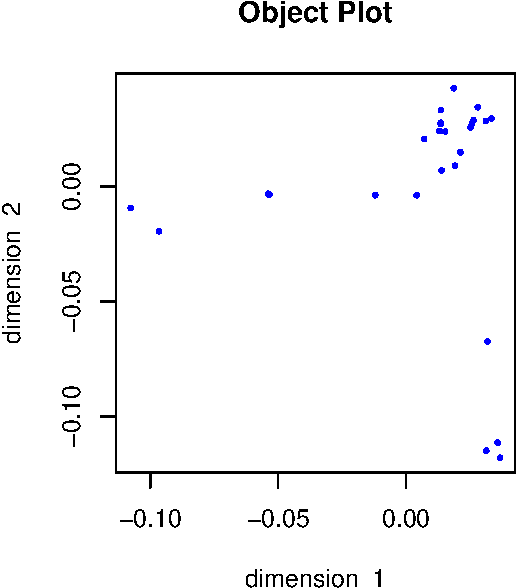
\includegraphics[keepaspectratio]{smacofHO_files/figure-latex/cetaplot-2.pdf}}

\begin{Shaded}
\begin{Highlighting}[]
\NormalTok{hcethopre }\OtherTok{\textless{}{-}} \FunctionTok{smacofPredictionTable}\NormalTok{(hcetho)}
\FunctionTok{print}\NormalTok{(}\FunctionTok{colSums}\NormalTok{(hcethopre, }\AttributeTok{na.rm =} \ConstantTok{TRUE}\NormalTok{))}
\end{Highlighting}
\end{Shaded}

\begin{verbatim}
##  [1] 33 15 35 33 28 25 28 25 23 36 29 35 16 22 28
\end{verbatim}

\begin{Shaded}
\begin{Highlighting}[]
\NormalTok{hcetno }\OtherTok{\textless{}{-}} \FunctionTok{smacofHO}\NormalTok{(cetacea, }\AttributeTok{verbose =} \ConstantTok{FALSE}\NormalTok{, }\AttributeTok{xnorm =} \DecValTok{2}\NormalTok{, }\AttributeTok{itmax =} \DecValTok{10000}\NormalTok{)}
\FunctionTok{smacofObjectsPlotHO}\NormalTok{(hcetno, }\AttributeTok{cex =}\NormalTok{ .}\DecValTok{5}\NormalTok{)}
\end{Highlighting}
\end{Shaded}

\pandocbounded{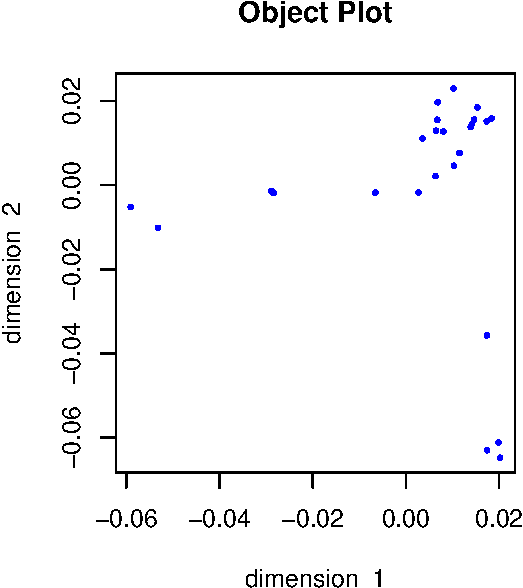
\includegraphics[keepaspectratio]{smacofHO_files/figure-latex/cetanorm-1.pdf}}

\begin{Shaded}
\begin{Highlighting}[]
\NormalTok{hcetnopre }\OtherTok{\textless{}{-}} \FunctionTok{smacofPredictionTable}\NormalTok{(hcetno)}
\FunctionTok{print}\NormalTok{(}\FunctionTok{sum}\NormalTok{(hcetnopre, }\AttributeTok{na.rm =} \ConstantTok{TRUE}\NormalTok{))}
\end{Highlighting}
\end{Shaded}

\begin{verbatim}
## [1] 404
\end{verbatim}

\subsection{Senate}\label{senate}

\begin{Shaded}
\begin{Highlighting}[]
\FunctionTok{data}\NormalTok{(senate, }\AttributeTok{package =} \StringTok{"homals"}\NormalTok{)}
\end{Highlighting}
\end{Shaded}

\begin{Shaded}
\begin{Highlighting}[]
\NormalTok{hhom }\OtherTok{\textless{}{-}} \FunctionTok{smacofHomogeneityHO}\NormalTok{(senate[, }\DecValTok{2}\SpecialCharTok{:}\DecValTok{21}\NormalTok{])}
\NormalTok{hho }\OtherTok{\textless{}{-}} \FunctionTok{smacofHO}\NormalTok{(senate[, }\DecValTok{2}\SpecialCharTok{:}\DecValTok{21}\NormalTok{], }\AttributeTok{verbose =} \ConstantTok{FALSE}\NormalTok{, }\AttributeTok{itmax =} \DecValTok{10000}\NormalTok{)}
\end{Highlighting}
\end{Shaded}

Stress is \ensuremath{2.0710178\times 10^{-7}} after 7449 iterations.

\begin{Shaded}
\begin{Highlighting}[]
\FunctionTok{smacofObjectsPlotHO}\NormalTok{(hhom, }\AttributeTok{cex =}\NormalTok{ .}\DecValTok{5}\NormalTok{, }\AttributeTok{labels =} \FunctionTok{as.character}\NormalTok{(senate[, }\DecValTok{1}\NormalTok{]))}
\end{Highlighting}
\end{Shaded}

\pandocbounded{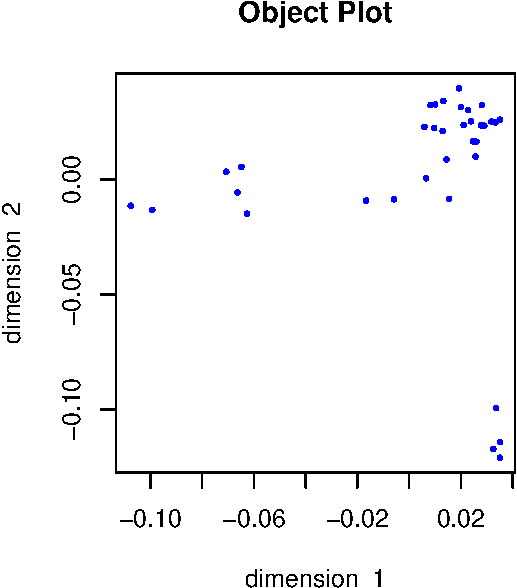
\includegraphics[keepaspectratio]{smacofHO_files/figure-latex/unnamed-chunk-1-1.pdf}}

\begin{Shaded}
\begin{Highlighting}[]
\NormalTok{hhompre }\OtherTok{\textless{}{-}} \FunctionTok{smacofPredictionTable}\NormalTok{(hhom)}
\FunctionTok{print}\NormalTok{(}\FunctionTok{colSums}\NormalTok{(hhompre, }\AttributeTok{na.rm =} \ConstantTok{TRUE}\NormalTok{))}
\end{Highlighting}
\end{Shaded}

\begin{verbatim}
##  [1]  93  95  97  88  89 100  99  97 100  96  98  91  96  85  89  87  89  86  86
## [20]  85
\end{verbatim}

\begin{Shaded}
\begin{Highlighting}[]
\FunctionTok{smacofObjectsPlotHO}\NormalTok{(hho, }\AttributeTok{cex =}\NormalTok{ .}\DecValTok{5}\NormalTok{, }\AttributeTok{labels =} \FunctionTok{as.character}\NormalTok{(senate[, }\DecValTok{1}\NormalTok{]))}
\end{Highlighting}
\end{Shaded}

\pandocbounded{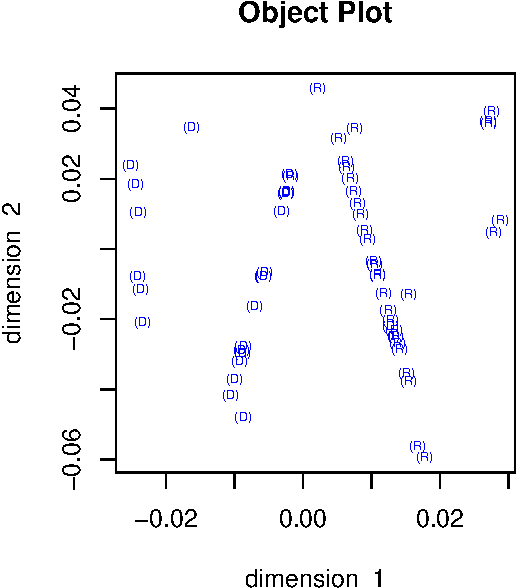
\includegraphics[keepaspectratio]{smacofHO_files/figure-latex/unnamed-chunk-1-2.pdf}}

\begin{Shaded}
\begin{Highlighting}[]
\NormalTok{hhopre }\OtherTok{\textless{}{-}} \FunctionTok{smacofPredictionTable}\NormalTok{(hho)}
\FunctionTok{print}\NormalTok{(}\FunctionTok{colSums}\NormalTok{(hhopre, }\AttributeTok{na.rm =} \ConstantTok{TRUE}\NormalTok{))}
\end{Highlighting}
\end{Shaded}

\begin{verbatim}
##  [1]  87  94  91  86  79 100  99  92 100  95  95  90  96  87  80  98  84  79 100
## [20]  79
\end{verbatim}

\begin{Shaded}
\begin{Highlighting}[]
\NormalTok{hno }\OtherTok{\textless{}{-}} \FunctionTok{smacofHO}\NormalTok{(senate[, }\DecValTok{2}\SpecialCharTok{:}\DecValTok{21}\NormalTok{], }\AttributeTok{verbose =} \ConstantTok{FALSE}\NormalTok{, }\AttributeTok{xnorm =} \DecValTok{2}\NormalTok{, }\AttributeTok{itmax =} \DecValTok{10000}\NormalTok{)}
\FunctionTok{smacofObjectsPlotHO}\NormalTok{(hno, }\AttributeTok{cex =}\NormalTok{ .}\DecValTok{5}\NormalTok{, }\AttributeTok{labels =} \FunctionTok{as.character}\NormalTok{(senate[, }\DecValTok{1}\NormalTok{]))}
\end{Highlighting}
\end{Shaded}

\pandocbounded{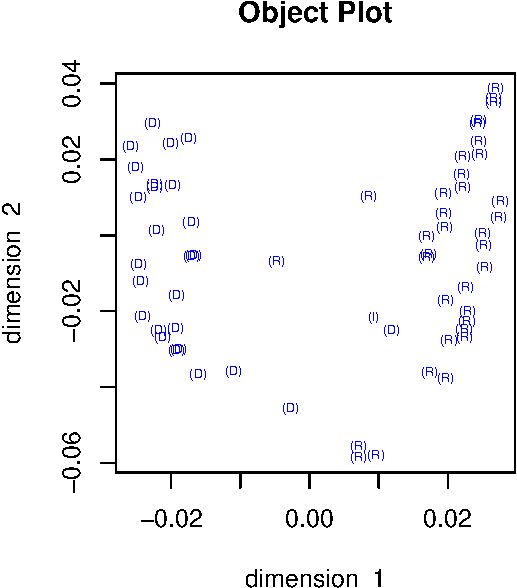
\includegraphics[keepaspectratio]{smacofHO_files/figure-latex/unnamed-chunk-2-1.pdf}}

\begin{Shaded}
\begin{Highlighting}[]
\NormalTok{hnopre }\OtherTok{\textless{}{-}} \FunctionTok{smacofPredictionTable}\NormalTok{(hno)}
\FunctionTok{print}\NormalTok{(}\FunctionTok{sum}\NormalTok{(hnopre, }\AttributeTok{na.rm =} \ConstantTok{TRUE}\NormalTok{))}
\end{Highlighting}
\end{Shaded}

\begin{verbatim}
## [1] 1833
\end{verbatim}

\subsection{GALO}\label{galo}

\begin{Shaded}
\begin{Highlighting}[]
\NormalTok{hgalohom }\OtherTok{\textless{}{-}} \FunctionTok{smacofHomogeneityHO}\NormalTok{(galo[, }\DecValTok{1}\SpecialCharTok{:}\DecValTok{4}\NormalTok{])}
\end{Highlighting}
\end{Shaded}

\begin{Shaded}
\begin{Highlighting}[]
\FunctionTok{smacofObjectsPlotHO}\NormalTok{(hgalohom, }\AttributeTok{cex =}\NormalTok{ .}\DecValTok{5}\NormalTok{)}
\end{Highlighting}
\end{Shaded}

\pandocbounded{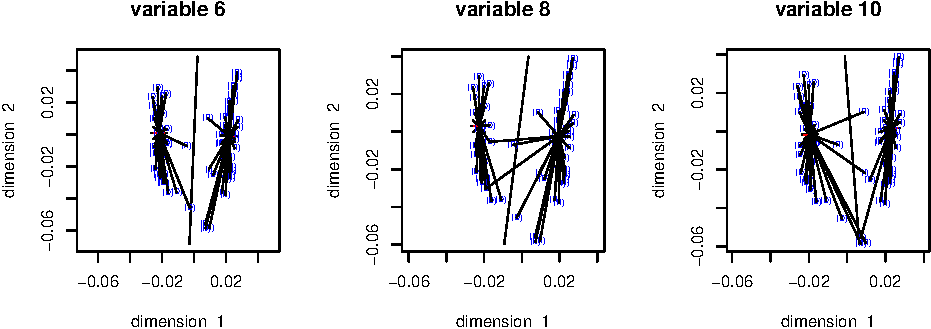
\includegraphics[keepaspectratio]{smacofHO_files/figure-latex/unnamed-chunk-3-1.pdf}}

\begin{Shaded}
\begin{Highlighting}[]
\NormalTok{hgalohompre }\OtherTok{\textless{}{-}} \FunctionTok{smacofPredictionTable}\NormalTok{(hgalohom)}
\FunctionTok{print}\NormalTok{(}\FunctionTok{colSums}\NormalTok{(hgalohompre, }\AttributeTok{na.rm =} \ConstantTok{TRUE}\NormalTok{))}
\end{Highlighting}
\end{Shaded}

\begin{verbatim}
## [1] 863 828 799 525
\end{verbatim}

\begin{Shaded}
\begin{Highlighting}[]
\FunctionTok{par}\NormalTok{(}\AttributeTok{mfrow =} \FunctionTok{c}\NormalTok{(}\DecValTok{1}\NormalTok{, }\DecValTok{2}\NormalTok{))}
\FunctionTok{smacofJointPlotsHO}\NormalTok{(hgalohom, }\AttributeTok{jvar =} \DecValTok{1}\SpecialCharTok{:}\DecValTok{2}\NormalTok{, }\AttributeTok{objects =} \ConstantTok{TRUE}\NormalTok{, }\AttributeTok{voronoi =} \ConstantTok{TRUE}\NormalTok{, }\AttributeTok{xcex =}\NormalTok{ .}\DecValTok{5}\NormalTok{, }\AttributeTok{ycex =}\NormalTok{ .}\DecValTok{5}\NormalTok{, }\AttributeTok{clabels =} \DecValTok{0}\NormalTok{)}
\end{Highlighting}
\end{Shaded}

\pandocbounded{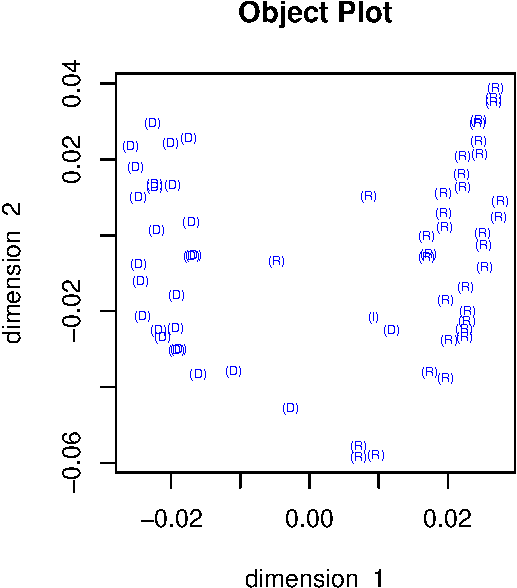
\includegraphics[keepaspectratio]{smacofHO_files/figure-latex/unnamed-chunk-4-1.pdf}}

\begin{Shaded}
\begin{Highlighting}[]
\NormalTok{hgaloho }\OtherTok{\textless{}{-}} \FunctionTok{smacofHO}\NormalTok{(galo[, }\DecValTok{1}\SpecialCharTok{:}\DecValTok{4}\NormalTok{], }\AttributeTok{verbose =} \ConstantTok{FALSE}\NormalTok{, }\AttributeTok{itmax =} \DecValTok{10000}\NormalTok{)}
\end{Highlighting}
\end{Shaded}

\begin{Shaded}
\begin{Highlighting}[]
\FunctionTok{smacofObjectsPlotHO}\NormalTok{(hgaloho, }\AttributeTok{cex =}\NormalTok{ .}\DecValTok{5}\NormalTok{)}
\end{Highlighting}
\end{Shaded}

\pandocbounded{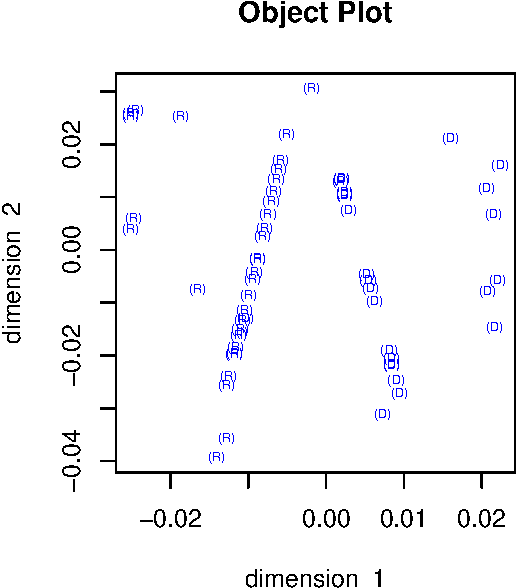
\includegraphics[keepaspectratio]{smacofHO_files/figure-latex/unnamed-chunk-5-1.pdf}}

\begin{Shaded}
\begin{Highlighting}[]
\NormalTok{hgalohopre }\OtherTok{\textless{}{-}} \FunctionTok{smacofPredictionTable}\NormalTok{(hgaloho)}
\FunctionTok{print}\NormalTok{(}\FunctionTok{colSums}\NormalTok{(hgalohopre, }\AttributeTok{na.rm =} \ConstantTok{TRUE}\NormalTok{))}
\end{Highlighting}
\end{Shaded}

\begin{verbatim}
## [1] 1290  397  921  385
\end{verbatim}

\begin{Shaded}
\begin{Highlighting}[]
\FunctionTok{par}\NormalTok{(}\AttributeTok{mfrow =} \FunctionTok{c}\NormalTok{(}\DecValTok{2}\NormalTok{, }\DecValTok{2}\NormalTok{))}
\FunctionTok{smacofJointPlotsHO}\NormalTok{(hgaloho, }\AttributeTok{objects =} \ConstantTok{TRUE}\NormalTok{, }\AttributeTok{voronoi =} \ConstantTok{TRUE}\NormalTok{, }\AttributeTok{xcex =}\NormalTok{ .}\DecValTok{5}\NormalTok{, }\AttributeTok{ycex =}\NormalTok{ .}\DecValTok{5}\NormalTok{, }\AttributeTok{clabels =} \DecValTok{0}\NormalTok{)}
\end{Highlighting}
\end{Shaded}

\pandocbounded{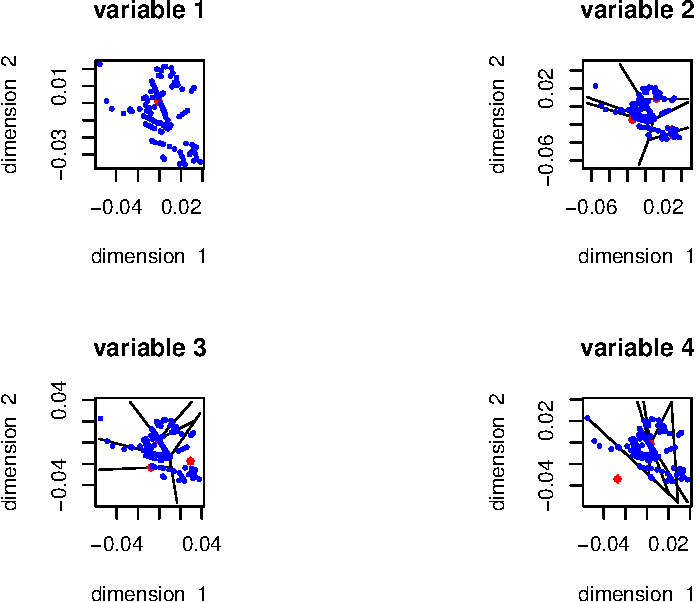
\includegraphics[keepaspectratio]{smacofHO_files/figure-latex/unnamed-chunk-6-1.pdf}}

\section{Generalizations}\label{generalizations}

\begin{enumerate}
\def\labelenumi{\arabic{enumi}.}
\tightlist
\item
  Fuzzy Indicators
\item
  Voronoi with general sites
\end{enumerate}

\section*{References}\label{references}
\addcontentsline{toc}{section}{References}

\phantomsection\label{refs}
\begin{CSLReferences}{1}{0}
\bibitem[\citeproctext]{ref-busing_10}
Busing, Frank M. T. A. 2010. {``Advances in Multidimensional Unfolding.''} PhD thesis, Leiden University.

\bibitem[\citeproctext]{ref-deleeuw_C_23}
De Leeuw, J. 1923. {``Deconstructing Multiple Correspondence Analysis. Essays in Honour of Shizuhiko Nishisato.''} In \emph{Analysis of Categorical Data from Historical Perspectives}, edited by Eric J. Beh, Rosaria Lombardo, and Jose G. Clavel, 383--407. Springer.

\bibitem[\citeproctext]{ref-deleeuw_R_69d}
---------. 1969. {``{Some Contributions to the Analysis of Categorical Data}.''} Research Note 004-69. Leiden, The Netherlands: Department of Data Theory FSW/RUL.

\bibitem[\citeproctext]{ref-deleeuw_A_77}
---------. 1977. {``Correctness of Kruskal's Algorithms for Monotone Regression with Ties.''} \emph{Psychometrika} 42: 141--44.

\bibitem[\citeproctext]{ref-deleeuw_U_03d}
---------. 2003. {``{Homogeneity Analysis Using Euclidean Minimum Spanning Trees}.''}

\bibitem[\citeproctext]{ref-deleeuw_R_04e}
---------. 2004. {``{Homogeneity Analysis of Pavings}.''} Preprint Series 389. Los Angeles, CA: UCLA Department of Statistics.

\bibitem[\citeproctext]{ref-deleeuw_C_14}
---------. 2014. {``{History of Nonlinear Principal Component Analysis}.''} In \emph{{The Visualization and Verbalization of Data}}, edited by J. Blasius and M. Greenacre. Chapman; Hall.

\bibitem[\citeproctext]{ref-deleeuw_heiser_C_80}
De Leeuw, J., and W. J. Heiser. 1980. {``Multidimensional Scaling with Restrictions on the Configuration.''} In \emph{Multivariate Analysis, Volume {V}}, edited by P. R. Krishnaiah, 501--22. Amsterdam, The Netherlands: North Holland Publishing Company.

\bibitem[\citeproctext]{ref-deleeuw_mair_A_09a}
De Leeuw, J., and P. Mair. 2009. {``{Homogeneity Analysis in {R}: the Package homals}.''} \emph{Journal of Statistical Software} 31 (4): 1--21. \url{https://www.jstatsoft.org/v31/i04/}.

\bibitem[\citeproctext]{ref-gifi_B_80}
Gifi, A. 1980. \emph{Niet-Lineaire Multivariate Analyse {[}Nonlinear Multivariate Analysis{]}}. Leiden, The Netherlands: Department of Data Theory FSW/RUL.

\bibitem[\citeproctext]{ref-gifi_B_90}
---------. 1990. \emph{Nonlinear Multivariate Analysis}. New York, N.Y.: Wiley.

\bibitem[\citeproctext]{ref-guttman_41}
Guttman, L. 1941. {``{The Quantification of a Class of Attributes: A Theory and Method of Scale Construction}.''} In \emph{The Prediction of Personal Adjustment}, edited by P. Horst, 321--48. New York: Social Science Research Council.

\bibitem[\citeproctext]{ref-guttman_85}
---------. 1985. {``Multidimensional Structuple Analysis (MSA-i) for the Classification ofCetacea: Whales, Porpoises and Dolphins.''} In \emph{Data Analysis in Real Life Environment: Ins and Outs of Solving Problems}, edited by J.-F. Marcotorchino, J. M. Proth, and J. Janssen. North-Holland.

\bibitem[\citeproctext]{ref-heiser_deleeuw_A_79}
Heiser, W. J., and J. De Leeuw. 1979. {``Metric Multidimensional Unfolding.''} \emph{Methoden En Data Nieuwsbrief SWS/VVS} 4: 26--50.

\bibitem[\citeproctext]{ref-hoffman_deleeuw_A_92}
Hoffman, D. L., and J. De Leeuw. 1992. {``Interpreting Multiple Correspondence Analysis as a Multidimensional Scaling Method.''} \emph{Marketing Letters} 3: 259--72.

\bibitem[\citeproctext]{ref-kruskal_64a}
Kruskal, J. B. 1964a. {``{Multidimensional Scaling by Optimizing Goodness of Fit to a Nonmetric Hypothesis}.''} \emph{Psychometrika} 29: 1--27.

\bibitem[\citeproctext]{ref-kruskal_64b}
---------. 1964b. {``{Nonmetric Multidimensional Scaling: a Numerical Method}.''} \emph{Psychometrika} 29: 115--29.

\bibitem[\citeproctext]{ref-kruskal_carroll_69}
Kruskal, J. B., and J. D. Carroll. 1969. {``{Geometrical Models and Badness of Fit Functions}.''} In \emph{Multivariate Analysis, Volume II}, edited by P. R. Krishnaiah, 639--71. North Holland Publishing Company.

\bibitem[\citeproctext]{ref-lingoes_68b}
Lingoes, J. C. 1968a. {``{The Multivariate Analysis Of Qualitative Data}.''} \emph{Multivariate Behavioral Research} 3 (1): 61--94.

\bibitem[\citeproctext]{ref-lingoes_68a}
---------. 1968b. {``{The Rationale of the Guttman-Lingoes Nonmetric Series: A Letter to Doctor Philip Runkel}.''} \emph{Multivariate Behavioral Research} 3 (4): 495--507.

\bibitem[\citeproctext]{ref-lingoes_72}
---------. 1972. {``A General Survey of the Guttman-Lingoes Nonmetric Program Series.''} In \emph{Multidimensional Scaling. Theory and Applications in the Behavioral Siences, Volume i, Theory}, edited by R. N. Shepard, A. K. Romney, and S. B. Nerlove, 52--68. Seminar Press.

\bibitem[\citeproctext]{ref-lingoes_73}
---------. 1973. \emph{{The Guttman-Lingoes Nonmetric Program Series}}. Mathesis Press.

\bibitem[\citeproctext]{ref-lingoes_79}
---------. 1979. {``Additional Programs in the Guttman-Lingoes Nonmetric Program Series: An Update.''} In \emph{{Geometric Representations of Relational Data}}, edited by J. C. Lingoes, Roskam E. E., and I. Borg, 283--87. Mathesis Press.

\bibitem[\citeproctext]{ref-marcotorchino_proth_janssen_85}
Marcotorchino, J.-F., J. M. Proth, and J. Janssen, eds. 1985. \emph{Data Analysis in Real Life Environment: Ins and Outs of Solving Problems}. North-Holland.

\bibitem[\citeproctext]{ref-michailidis_deleeuw_A_98}
Michailidis, G., and J. De Leeuw. 1998. {``The Gifi System for Descriptive Multivariate Analysis.''} \emph{Statistical Science} 13: 307--36.

\bibitem[\citeproctext]{ref-roskam_68}
Roskam, E. E. 1968. {``{Metric Analysis of Ordinal Data in Psychology}.''} PhD thesis, University of Leiden.

\bibitem[\citeproctext]{ref-vanderburg_85}
Van der Burg, E. 1985. {``HOMALS Classification of Whales, Porpoises and Dolphins.''} In \emph{Data Analysis in Real Life Environment: Ins and Outs of Solving Problems}, edited by J.-F. Marcotorchino, J. M. Proth, and J. Janssen. North-Holland.

\bibitem[\citeproctext]{ref-vandeun_05}
Van Deun, Katrijn. 2005. {``Degeneracies in Multidimensional Scaling.''} PhD thesis, KU Leuven.

\bibitem[\citeproctext]{ref-vescia_85}
Vescia, G. 1985. {``Descriptive Classification of Cetacea: Whales, Porpoises and Dolphins.''} In \emph{Data Analysis in Real Life Environment: Ins and Outs of Solving Problems}, edited by J.-F. Marcotorchino, J. M. Proth, and J. Janssen, 7--13. North-Holland.

\bibitem[\citeproctext]{ref-zvulun_78}
Zvulun, Eli. 1978. {``Multidimensional Scalogram Analysis:the Method and Its Application.''} In \emph{Theory Construction and Data Analysis in the Behavioral Sciences}, edited by Samuel Shye, 237--64. Jossey-Bass.

\end{CSLReferences}

\end{document}
